% Created 2023-03-27 Mon 01:58
% Intended LaTeX compiler: lualatex
\documentclass[bigger]{beamer}
\usepackage{graphicx}
\usepackage{longtable}
\usepackage{wrapfig}
\usepackage{rotating}
\usepackage[normalem]{ulem}
\usepackage{amsmath}
\usepackage{amssymb}
\usepackage{capt-of}
\usepackage{hyperref}
\usetheme[progressbar=foot, sectionpage=none, numbering=fraction]{metropolis}
\usepackage{tikz}
\usepackage{booktabs}
\usepackage{adjustbox}
\usepackage{diagbox}
\usepackage{latexcolors}
\usetikzlibrary{automata, positioning, arrows, arrows.meta}
\usepackage{diagbox}
\usepackage{dsfont}
\usepackage{amsmath}
\usepackage{fontawesome5}
\usepackage{color}
\usepackage{transparent}
\usepackage{textpos}
\definecolor{RedBrown}{RGB}{192, 4, 4} \setbeamercolor{progress bar}{fg=RedBrown} \setbeamercolor{title separator}{fg=RedBrown}
\setbeamercolor{progress bar in head/foot}{fg=RedBrown} \setbeamercolor{progress bar in section page}{fg=RedBrown} \setbeamercolor{alerted text}{fg=RedBrown}
\pretocmd{\tableofcontents}{\thispagestyle{empty}}{}{}
\addtocounter{framenumber}{-1}
\usepackage{listings}
\usepackage{xcolor}
\definecolor{codegreen}{rgb}{0,0.6,0}
\definecolor{codegray}{rgb}{0.5,0.5,0.5}
\definecolor{codepurple}{rgb}{0.58,0,0.82}
\definecolor{backcolour}{HTML}{f0f0f0}
\lstdefinestyle{mystyle}{
backgroundcolor=\color{backcolour},
commentstyle=\color{codegreen},
keywordstyle=\color{magenta},
numberstyle=\tiny\color{codegray},
stringstyle=\color{codepurple},
basicstyle=\ttfamily,
breakatwhitespace=false,
breaklines=true,
captionpos=b,
keepspaces=true,
numbers=none,
numbersep=5pt,
showspaces=false,
showstringspaces=false,
showtabs=false,
tabsize=2
}
\lstset{style=mystyle}
\usetheme{default}
\author{Andrea Pierré}
\date{April 4\textsuperscript{th}, 2023}
\title{NSGP seminar}
\subtitle{Learning useful representations to solve a place-odor association task}
\institute{Brown University}
\titlegraphic{\hfill
\includegraphics[height=1.5cm]{img/Brown Logo_2016_2 Color Process ST_1300.png}}
\setbeamercovered{transparent=10}
\setbeamertemplate{section in toc}[sections numbered]
\AtBeginSection[]{\begin{frame}[plain, noframenumbering]{Outline}    \setbeamertemplate{section in toc}[sections numbered]\setbeamertemplate{subsection in toc}[subsections numbered]\tableofcontents[currentsection, currentsubsection]\end{frame}}
\AtBeginSubsection[]{\begin{frame}[plain, noframenumbering]{Outline}\setbeamertemplate{section in toc}[sections numbered]\setbeamertemplate{subsection in toc}[subsections numbered]\tableofcontents[currentsection,currentsubsection]\end{frame}}
\begin{document}

\maketitle
\begin{frame}[plain]{Outline}
\tableofcontents
\end{frame}

\section{Context of the project}
\label{sec:orgd4e5f00}
\begin{frame}[label={sec:org53479a5}]{Why we record in the LEC?}
\begin{itemize}
\item Hypothesised to encode local
\end{itemize}
\end{frame}
\begin{frame}[label={sec:org5b444a4}]{Joint representation}
\begin{block}{Feature selection}
\begin{itemize}
\item Which features/representations are needed/the brain use to learn the task?
\end{itemize}
\end{block}
\end{frame}
\begin{frame}[label={sec:orgd683ae6}]{What is Reinforcement Learning and why we want to use it ?}
\begin{columns}
\begin{column}{0.6\columnwidth}
% \usepackage{fontawesome5}
\usetikzlibrary{positioning,fit,arrows}


\tikzset{
    %Define standard arrow tip
    >=latex,
    %Define style for boxes
    punkt/.style={
           rectangle,
           rounded corners,
           draw=black, very thick,
           text width=7.5em,
           minimum height=2em,
           text centered},
    % Define arrow style
    pil/.style={
           ->,
           thick,}
}

\begin{adjustbox}{max width=\columnwidth, keepaspectratio}
    \begin{tikzpicture}[node distance=3em, auto,]
     %nodes
        \node (center) {};
        \node[punkt, above=of center] (agent) {Agent \faIcon{robot}};
        \node[punkt,below=of center] (environment) {Environment \faIcon{globe}};
        \node[right=8em of center, align=center] (action) {Action\\$a_t$};
        \node[left=8em of center, align=center] (state_reward) {State, Reward\\$s_t$, $r_t$};

        \path[pil]
        (state_reward.east) edge [->, bend left=45] node {} (agent.west)
        (environment.west) edge [- , bend left=45] node {} (state_reward.east)
        (action.west) edge [->, bend left=45] node {} (environment.east)
        (agent.east) edge [-, bend left=45] node {} (action.west);
    \end{tikzpicture}
\end{adjustbox}
\end{column}

\begin{column}{0.4\columnwidth}
\small
\begin{itemize}
\item Goal of the agent : maximize rewards
\item Natural fit for behavioral experiments involving rewards and learning
\end{itemize}
\end{column}
\end{columns}
\end{frame}

\begin{frame}[label={sec:orgc5901be}]{Temporal Difference learning}
\begin{columns}
\begin{column}{0.5\columnwidth}
\begin{center}
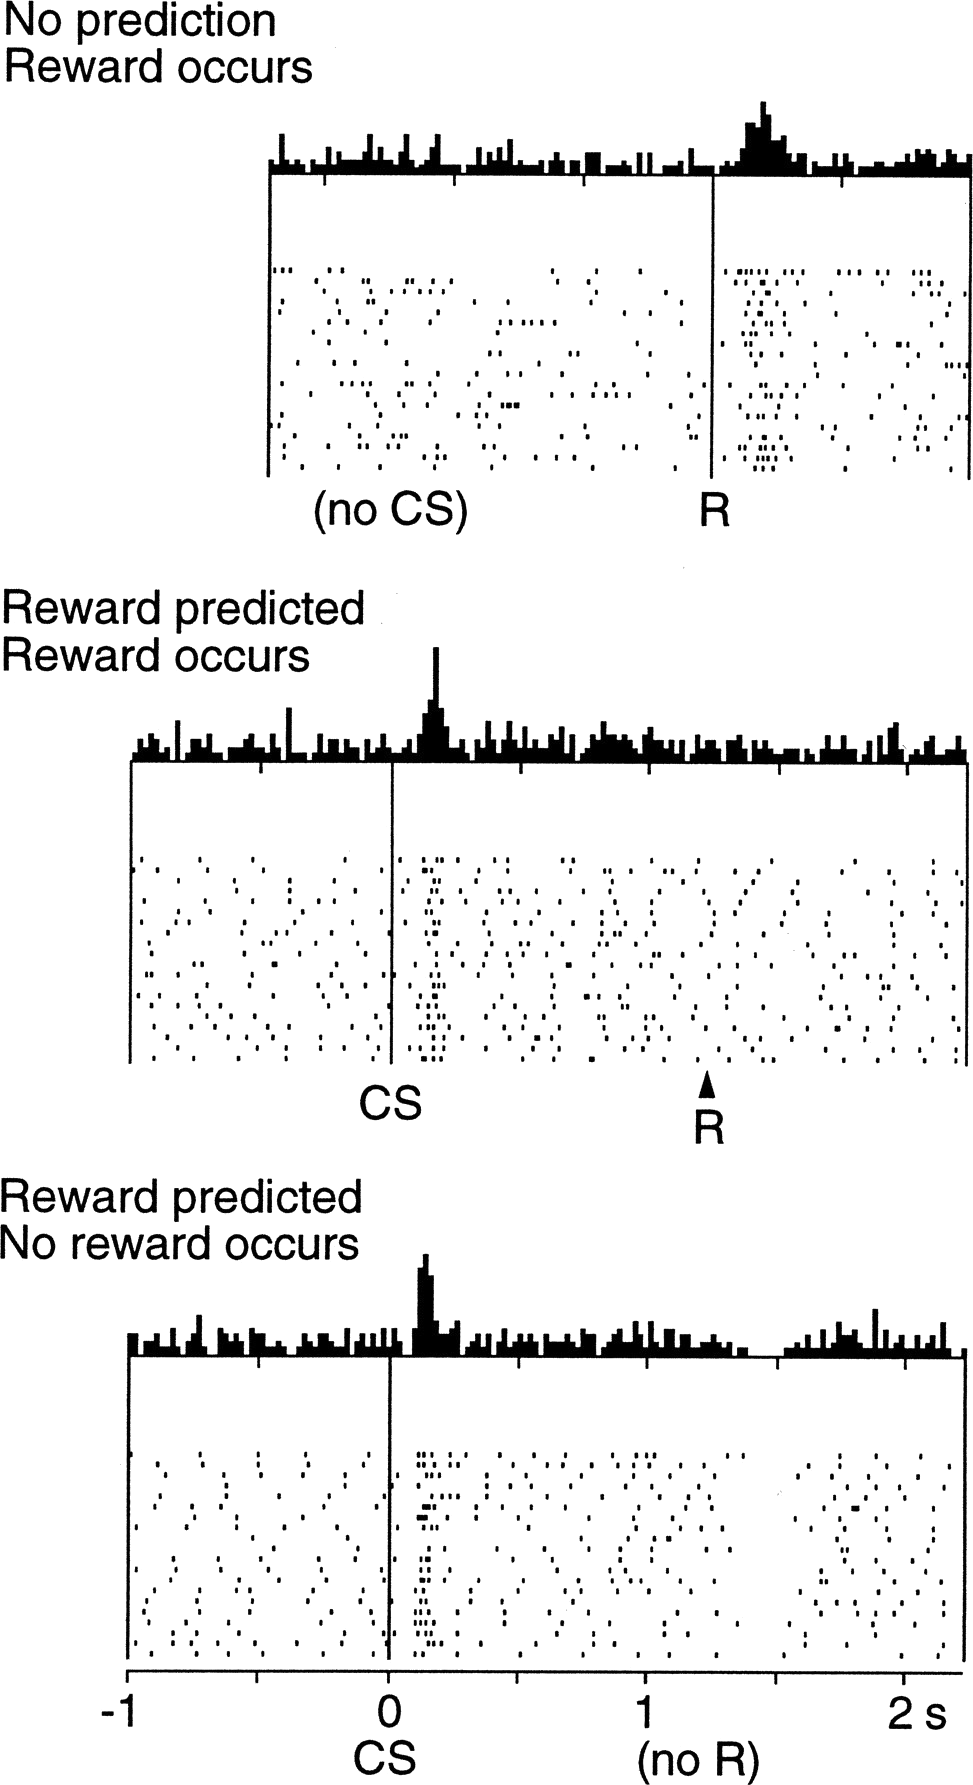
\includegraphics[height=0.8\textheight]{./img/Schultz et al. (1997).png}
\end{center}
Schultz et al. (1997)
\end{column}
\begin{column}{0.5\columnwidth}
\begin{adjustbox}{max width=\columnwidth, keepaspectratio}
$V(S_t) = V(S_t) + \alpha(\underbrace{R_{t+1} + \gamma V(S_{t+1})}_\text{TD target} - V(S_t))$
\end{adjustbox}\\[1em]
\begin{adjustbox}{max width=\columnwidth, keepaspectratio}
$NewEstimate \leftarrow OldEstimate + StepSize[Target - OldEstimate]$
\end{adjustbox}
\end{column}
\end{columns}
\end{frame}
\begin{frame}[label={sec:org5707c59}]{Hypothesis}
\metroset{block=fill}
\begin{exampleblock}{Hypothesis}
LEC hypothesized to encode the conjunction of odor-place information
\end{exampleblock}
\end{frame}
\section{Experimental setup and task}
\label{sec:orgf95b7e8}
\begin{frame}[label={sec:orgbbaad3c}]{Olivia's diamond arena olfactory task}
\begin{columns}
\begin{column}[t]{0.5\columnwidth}
\center
Allocentric\\
(go west/east)
\begin{center}
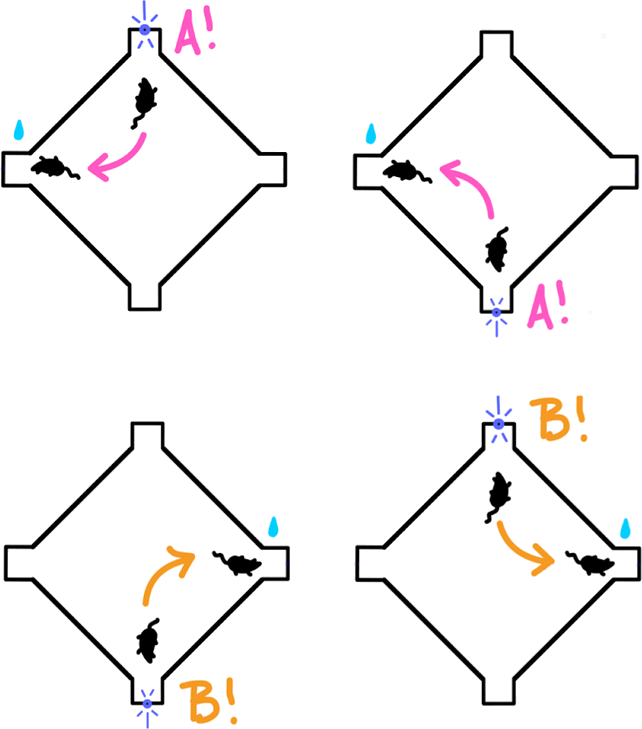
\includegraphics[width=0.8\textwidth]{img/allocentric-task.png}
\end{center}
\end{column}

\begin{column}[t]{0.5\columnwidth}
\center
Egocentric\\
(go right/left)
\begin{center}
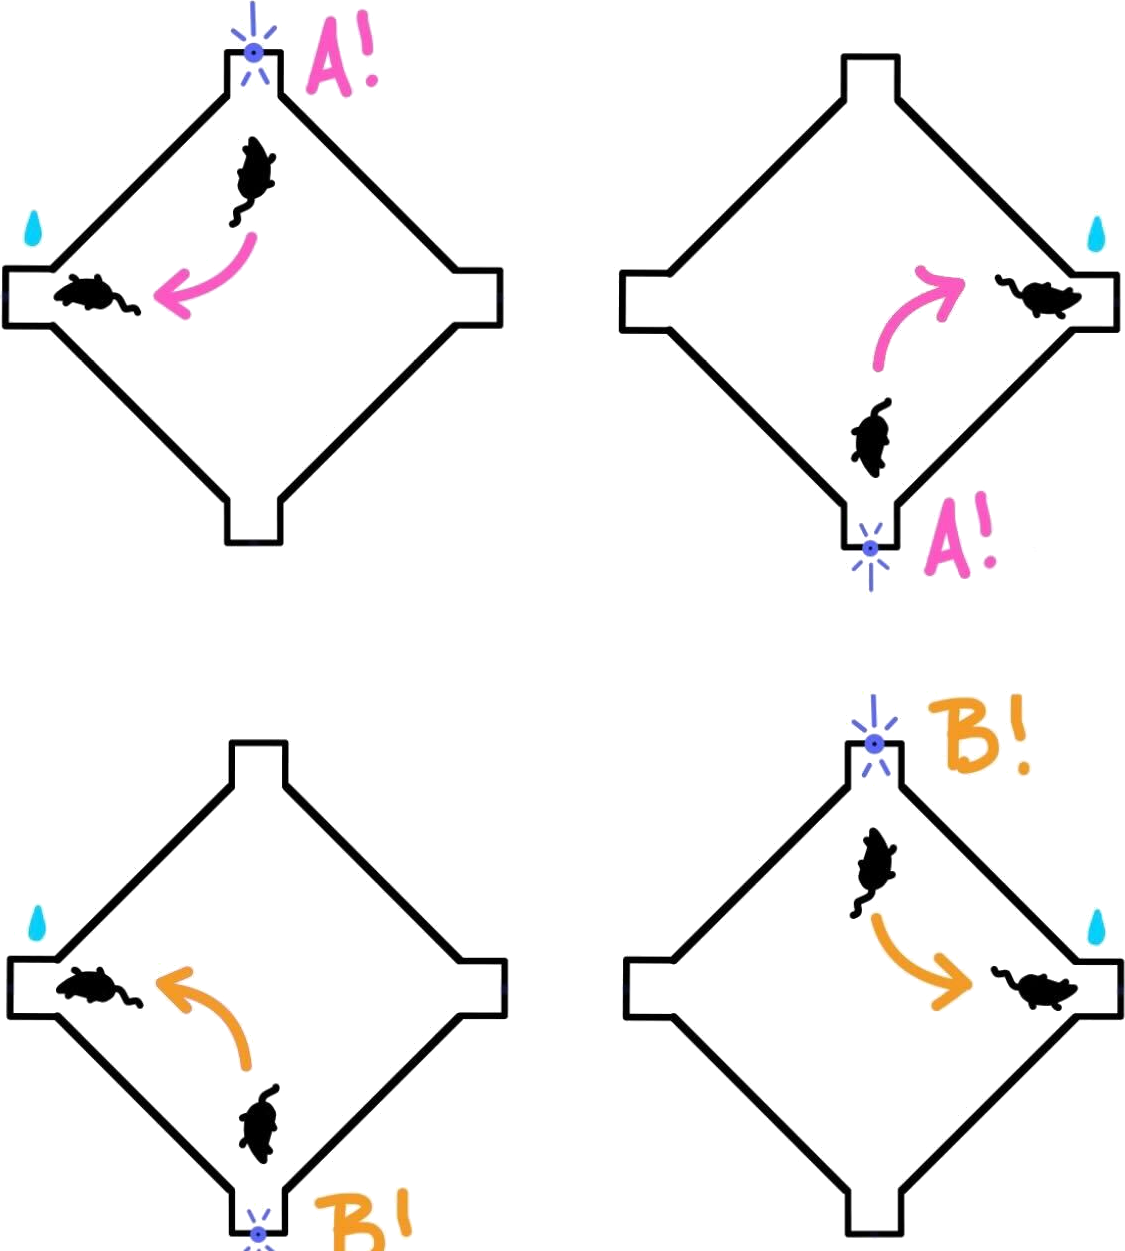
\includegraphics[width=0.8\textwidth]{img/egocentric-task.png}
\end{center}

\begin{textblock}{5}(-1,13)
\center
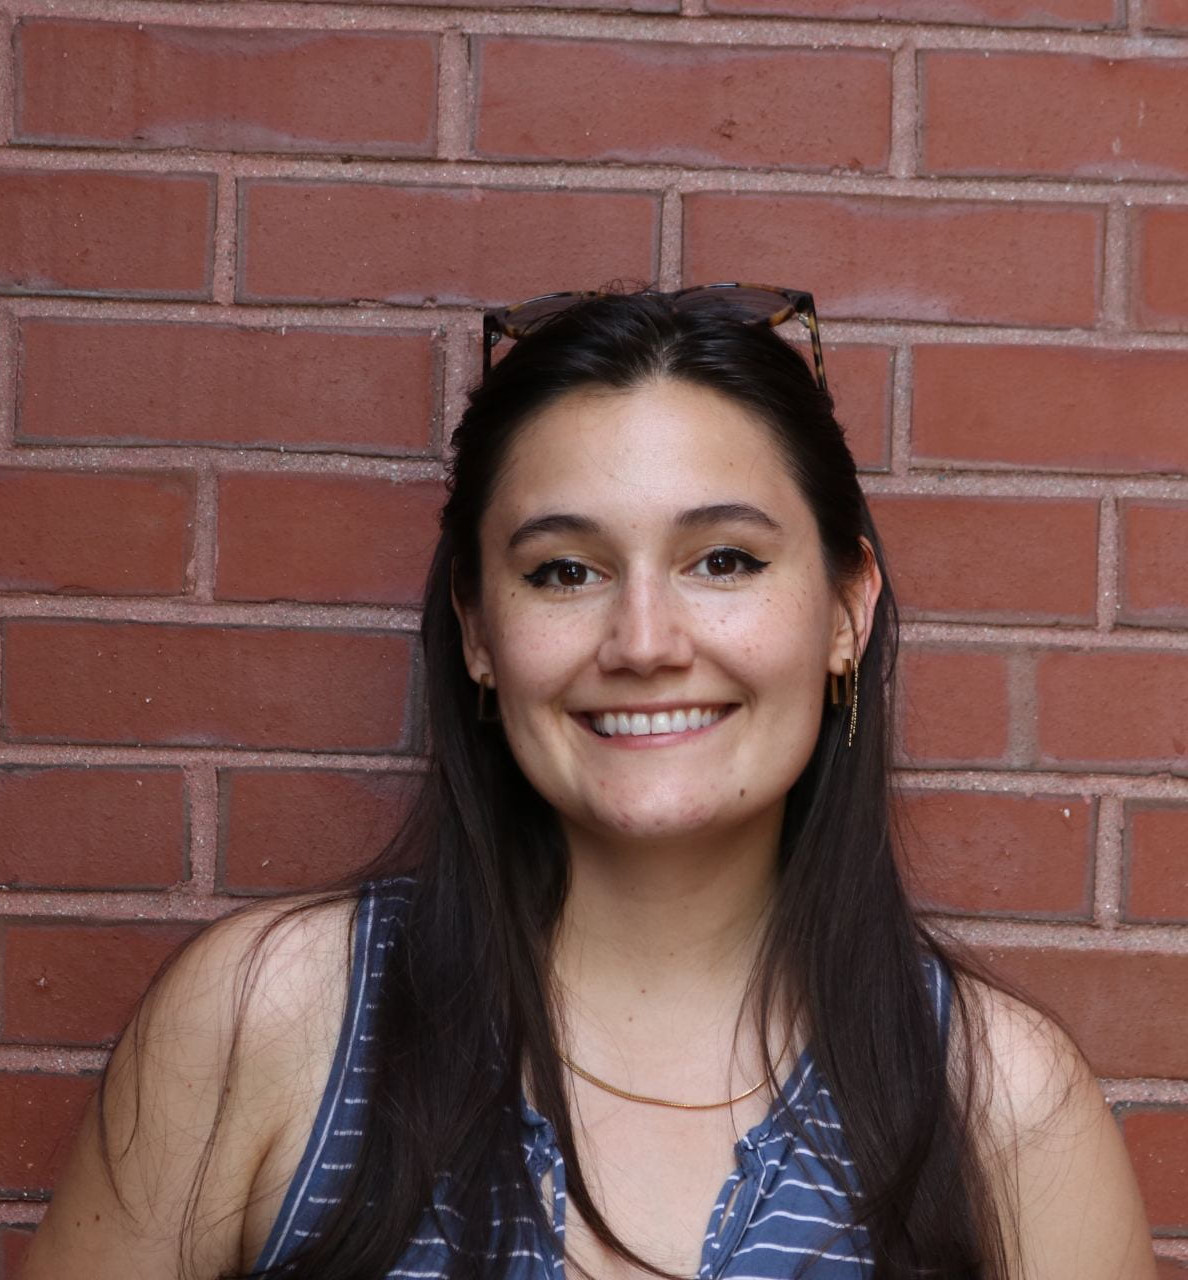
\includegraphics[width=3em]{img/olivia.jpg}\\
\scriptsize
Olivia McKissick
\end{textblock}
\end{column}
\end{columns}
\end{frame}

\begin{frame}[label={sec:orgad6fe7e}]{Diamond arena experimental setup}
\begin{center}
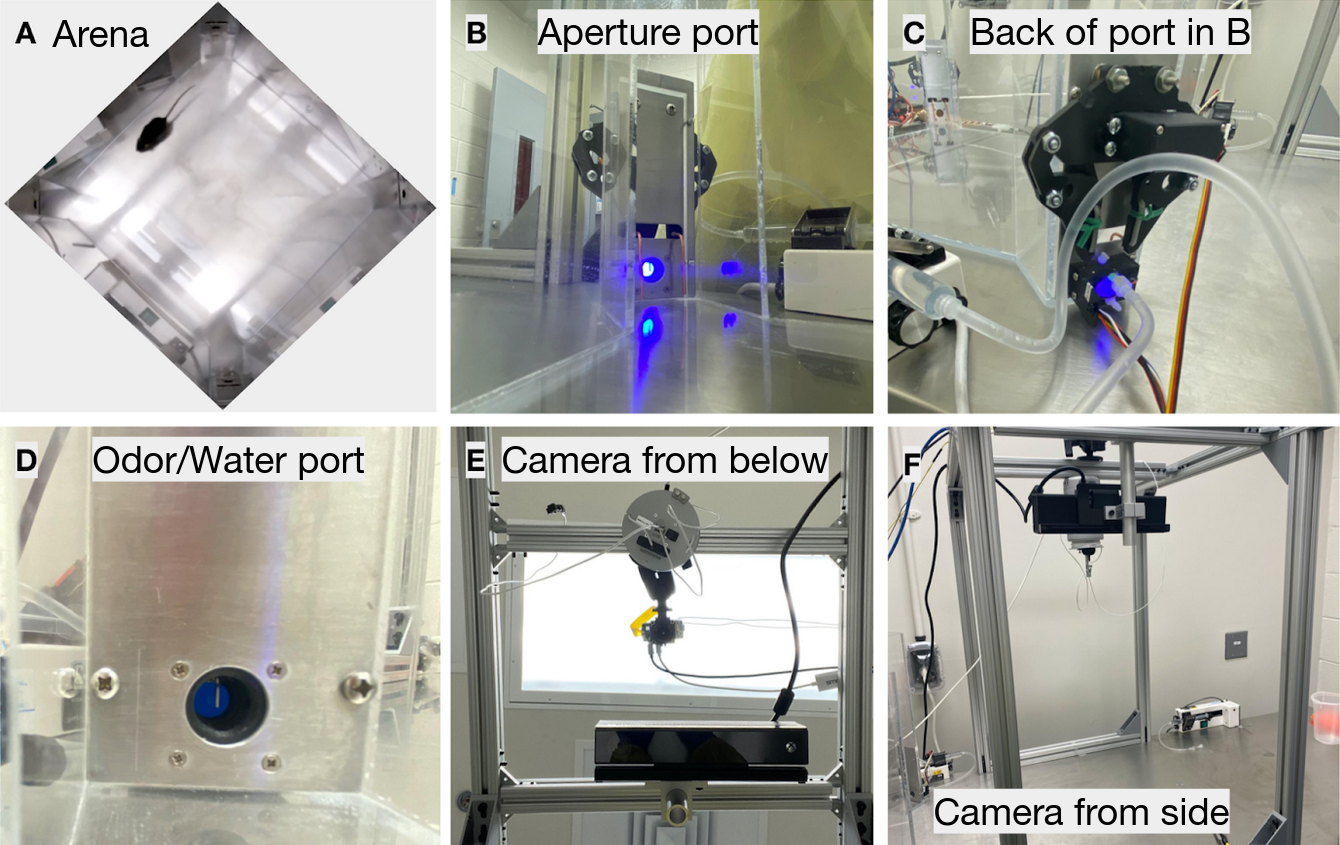
\includegraphics[width=.9\linewidth]{img/physical-diamond-arena.png}
\end{center}
\end{frame}
\section{Experiments \& preliminary results}
\label{sec:org475ebd5}
\begin{frame}[label={sec:org9c5eeba}]{The model}
\begin{columns}
\begin{column}{0.5\columnwidth}
\center
Allocentric
\begin{center}
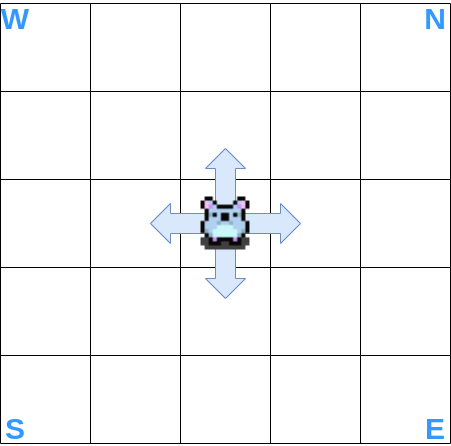
\includegraphics[width=\textwidth]{img/RL_environment-Allo.drawio.png}
\end{center}
\end{column}
\begin{column}{0.5\columnwidth}
\center
Egocentric
\begin{center}
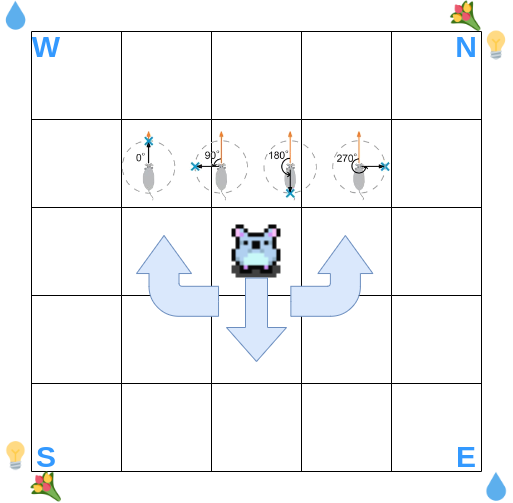
\includegraphics[width=\textwidth]{img/RL_environment-Ego.drawio.png}
\end{center}
\end{column}
\end{columns}
\end{frame}
\begin{frame}[label={sec:org1d842ec}]{Without joint representation}
\begin{columns}
\begin{column}{0.5\columnwidth}
\begin{center}
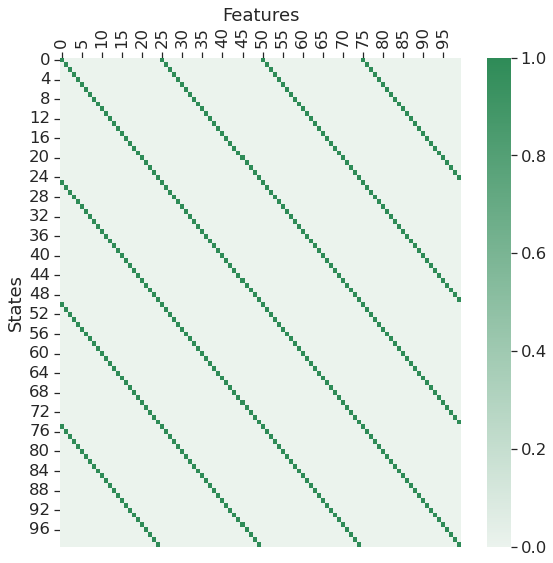
\includegraphics[height=0.4\textheight]{img/features-allo-no-joint-repr.png}
\end{center}
\end{column}
\begin{column}{0.5\columnwidth}
\begin{center}
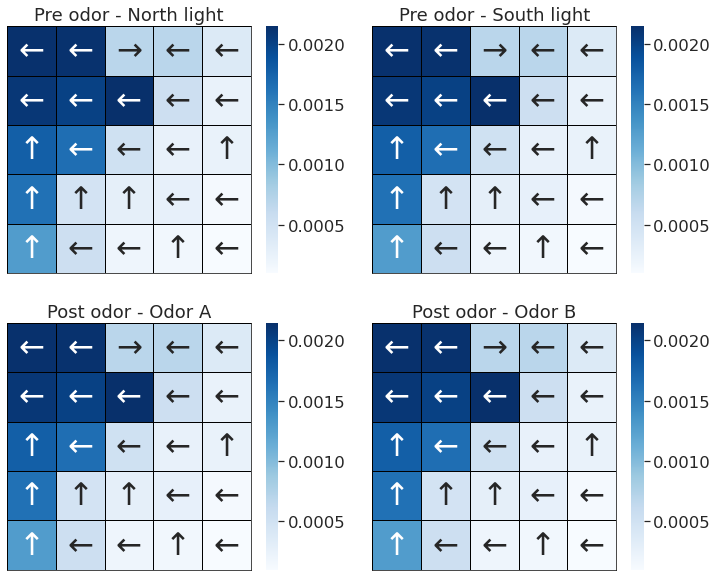
\includegraphics[width=\textwidth]{img/policy-allo-no-joint-repr.png}
\end{center}
\end{column}
\end{columns}
\begin{block}{~}
\vspace{-2em}
\begin{center}
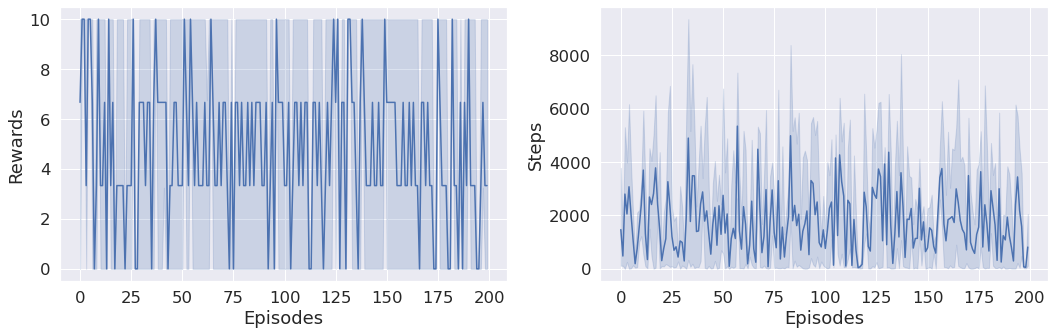
\includegraphics[height=0.4\textheight]{img/rewards-steps-allo-no-joint-repr.png}
\end{center}
\(\to\) The agent is unable to solve the task
\end{block}
\end{frame}
\begin{frame}[label={sec:org0d39be9}]{With joint representation}
\begin{columns}
\begin{column}{0.5\columnwidth}
\begin{center}
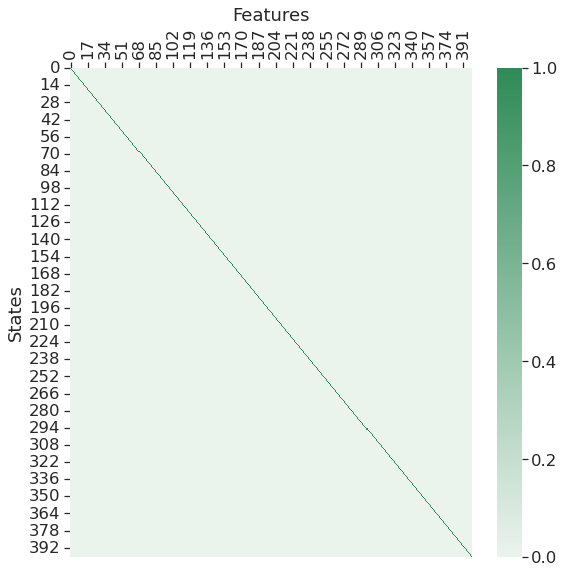
\includegraphics[height=0.4\textheight]{img/features-ego-joint-repr.png}
\end{center}
\end{column}
\begin{column}{0.5\columnwidth}
\begin{center}
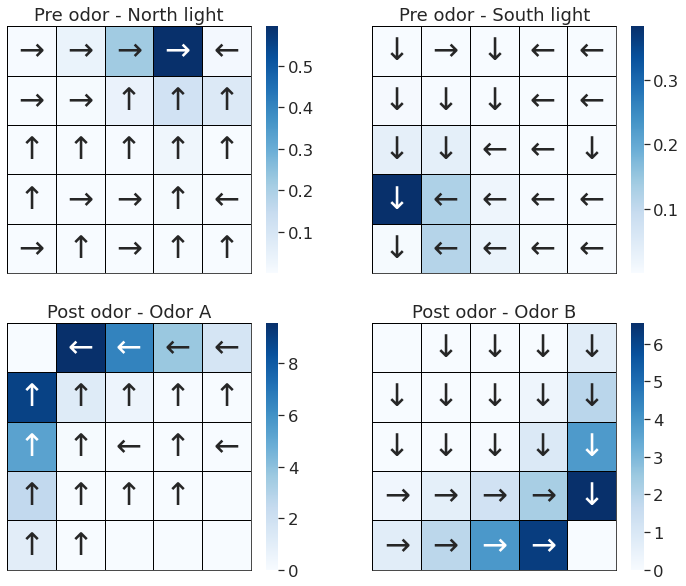
\includegraphics[width=\textwidth]{img/policy-allo-joint-repr.png}
\end{center}
\end{column}
\end{columns}
\begin{block}{~}
\vspace{-2em}
\begin{center}
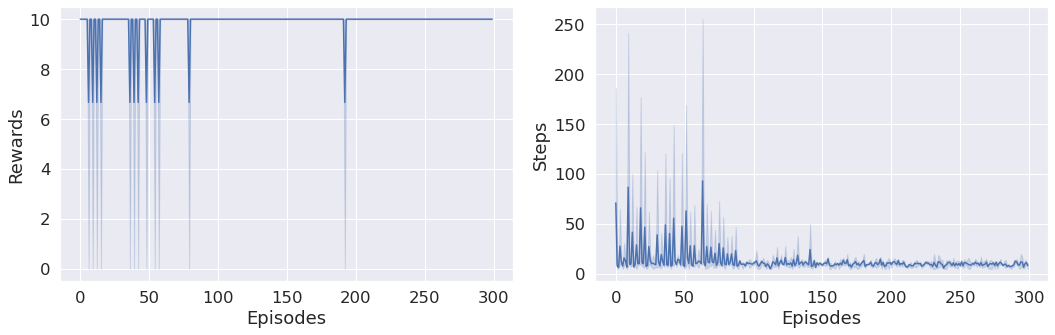
\includegraphics[height=0.4\textheight]{img/rewards-steps-allo-joint-repr.png}
\end{center}
\(\to\) The agent learns to solve the task
\end{block}
\end{frame}
\begin{frame}[label={sec:orgc85aed6}]{States occupancy ?}
\end{frame}
\begin{frame}[label={sec:orge816f9f}]{Can we predict the behavioral data ?}
\begin{center}
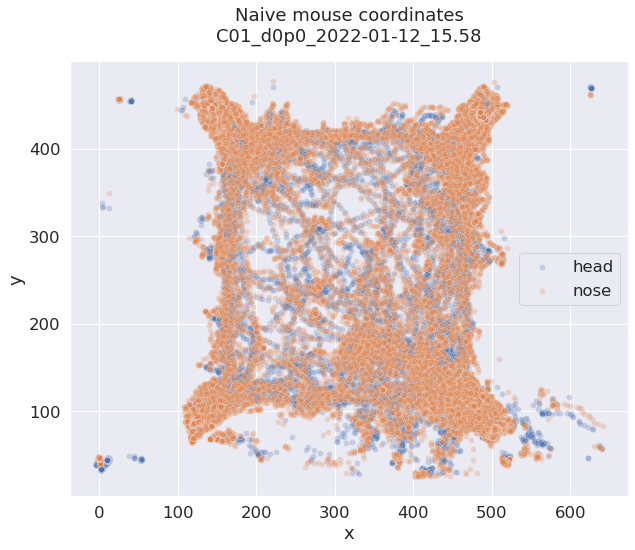
\includegraphics[width=.9\linewidth]{img/naive-mouse-coords.png}
\end{center}
\end{frame}
\section{What we plan to do next}
\label{sec:org4003d66}
\begin{frame}[label={sec:orgdafad52}]{What we plan to do next}
\end{frame}
\begin{frame}[label={sec:orgdde472e}]{From tabular RL to deep RL}
% \usepackage{fontawesome5}
\usetikzlibrary{positioning,fit,arrows}


\tikzset{
    %Define standard arrow tip
    >=latex,
    %Define style for boxes
    punkt/.style={
           rectangle,
           rounded corners,
           draw=black, very thick,
           text width=7.5em,
           minimum height=2em,
           text centered},
    % Define arrow style
    pil/.style={
           ->,
           thick,}
}

\begin{adjustbox}{max height=\textheight, keepaspectratio}
    \begin{tikzpicture}[node distance=3em, auto,]
     %nodes
        \node (center) {};
        \node[punkt, above=of center] (agent) {Agent \faIcon{robot}};
        % \node at (0,3.7) {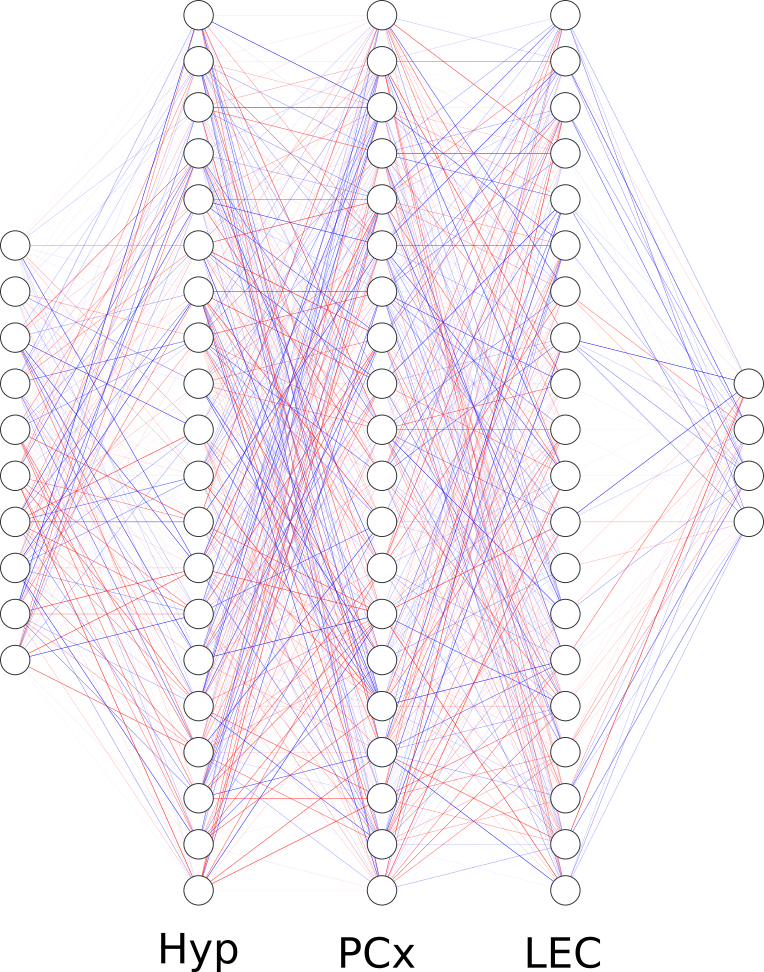
\includegraphics[height=6em]{./img/nn.svg.png}};
        \node [above=-0.2em of agent] {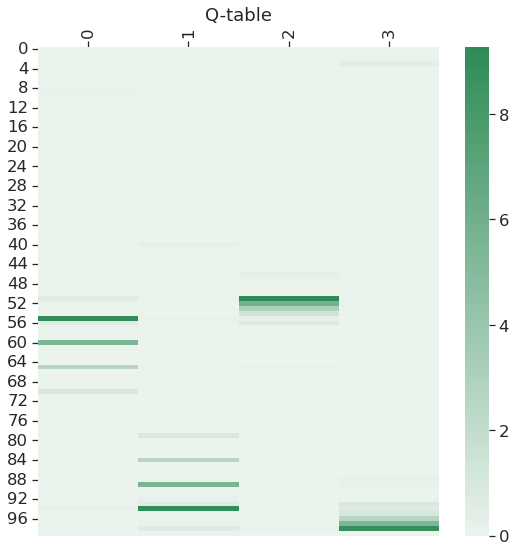
\includegraphics[height=6em]{./img/Q-table.png}};
        \node[punkt,below=of center] (environment) {Environment \faIcon{globe}};
        \node[right=8em of center, align=center] (action) {Action\\$a_t$};
        \node[left=8em of center, align=center] (state_reward) {State, Reward\\$s_t$, $r_t$};
        \node [below=-0.2em of environment] {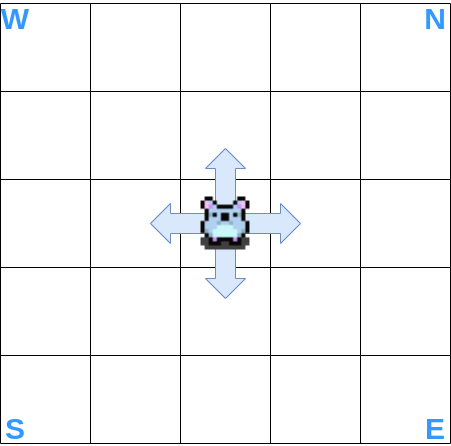
\includegraphics[height=6em]{./img/RL_environment-Allo.drawio.png}};

        \path[pil]
        (state_reward.east) edge [->, bend left=45] node {} (agent.west)
        (environment.west) edge [- , bend left=45] node {} (state_reward.east)
        (action.west) edge [->, bend left=45] node {} (environment.east)
        (agent.east) edge [-, bend left=45] node {} (action.west);
    \end{tikzpicture}
\end{adjustbox}
\end{frame}

\begin{frame}[label={sec:orgcba9214}]{From tabular RL to deep RL}
% \usepackage{fontawesome5}
\usetikzlibrary{positioning,fit,arrows}


\tikzset{
    %Define standard arrow tip
    >=latex,
    %Define style for boxes
    punkt/.style={
           rectangle,
           rounded corners,
           draw=black, very thick,
           text width=7.5em,
           minimum height=2em,
           text centered},
    % Define arrow style
    pil/.style={
           ->,
           thick,}
}

\begin{adjustbox}{max height=\textheight, keepaspectratio}
    \begin{tikzpicture}[node distance=3em, auto,]
     %nodes
        \node (center) {};
        \node[punkt, above=of center] (agent) {Agent \faIcon{robot}};
        % \node at (0,3.7) {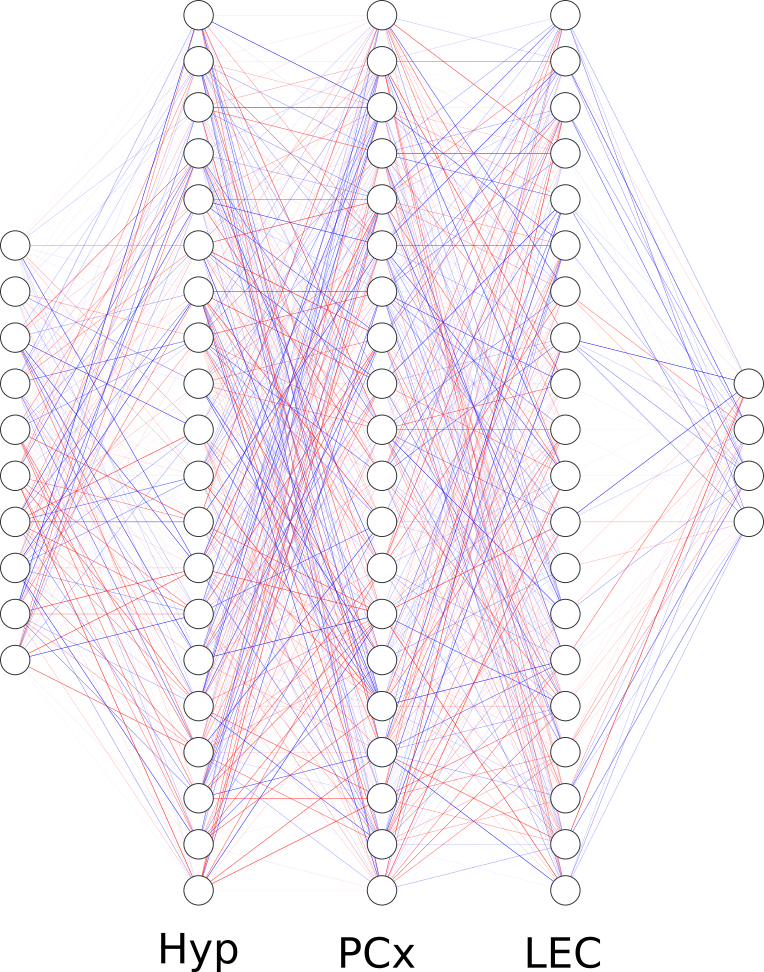
\includegraphics[height=6em]{./img/nn.svg.png}};
        \node [above=-0.2em of agent] {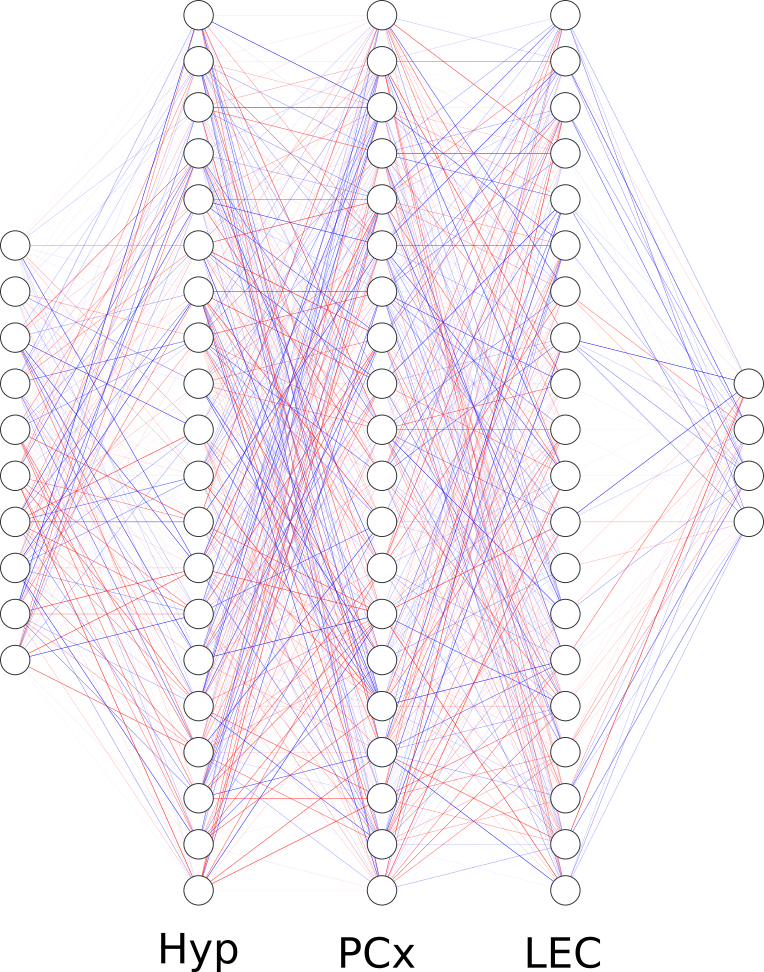
\includegraphics[height=6em]{./img/nn.svg.png}};
        \node[punkt,below=of center] (environment) {Environment \faIcon{globe}};
        \node[right=8em of center, align=center] (action) {Action\\$a_t$};
        \node[left=8em of center, align=center] (state_reward) {State, Reward\\$s_t$, $r_t$};
        \node [below=-0.2em of environment] {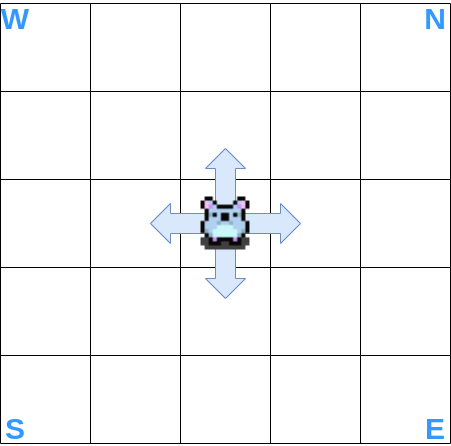
\includegraphics[height=6em]{./img/RL_environment-Allo.drawio.png}};

        \path[pil]
        (state_reward.east) edge [->, bend left=45] node {} (agent.west)
        (environment.west) edge [- , bend left=45] node {} (state_reward.east)
        (action.west) edge [->, bend left=45] node {} (environment.east)
        (agent.east) edge [-, bend left=45] node {} (action.west);
    \end{tikzpicture}
\end{adjustbox}
\end{frame}

\begin{frame}[label={sec:orgcd13342}]{What we expect to see}
\begin{columns}
\begin{column}{0.5\columnwidth}
% \begin{adjustbox}{max width=\columnwidth, keepaspectratio}
% Approximate the value function with a \alert{basis function}~:
% \end{adjustbox}
% \begin{adjustbox}{max width=\columnwidth, keepaspectratio}
% \(\hat{\upsilon}(s, \mathrm{\mathbf{w}}) \: \dot{=} \: \mathrm{\mathbf{w}}^T \mathrm{\mathbf{x}}(s) \: \dot{=} \: \displaystyle\sum_{i=1}^{d}  w_i x_i(s)\)
% \end{adjustbox}\\[1em]
% \begin{adjustbox}{max width=\columnwidth, keepaspectratio}
% \(
%   \begin{aligned}
% \hat{\upsilon} &: \text{approximate value of state $s$ given weight vector $w$}\\
% s &: \text{state}\\
% \mathrm{\mathbf{w}} &: \text{$d$-vector of weights underlying the approximate value function}\\
% \mathrm{\mathbf{x}} &: \text{vector of features visible when in state $s$}\\
% w &: \text{$i$th component of learnable weight vector}\\
% x &: \text{$i$th component of vector $x(s)$}\\
%   \end{aligned}
% \)
% \end{adjustbox}
\end{column}
\begin{column}{0.5\columnwidth}
\center
\scriptsize
Find some candidate patterns in the data~: place cells, grid cells~?
\normalsize
\begin{center}
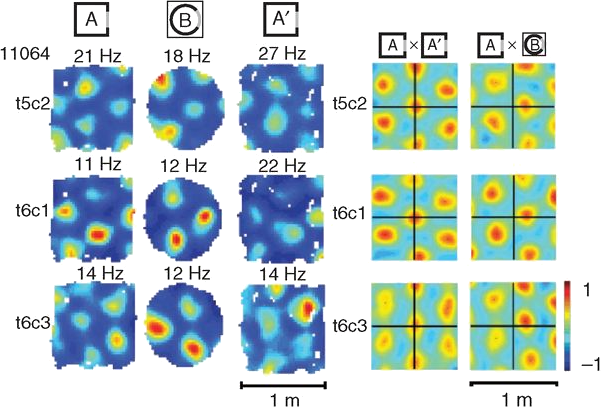
\includegraphics[height=0.25\textheight]{img/place-cells-grid-cells.jpg.png}
\end{center}

% \center
% \scriptsize
% Approximate with coarse coding ? Tiling ?
% \normalsize

\begin{textblock}{5}(0,12)
\begin{minipage}[t]{3em}
\center
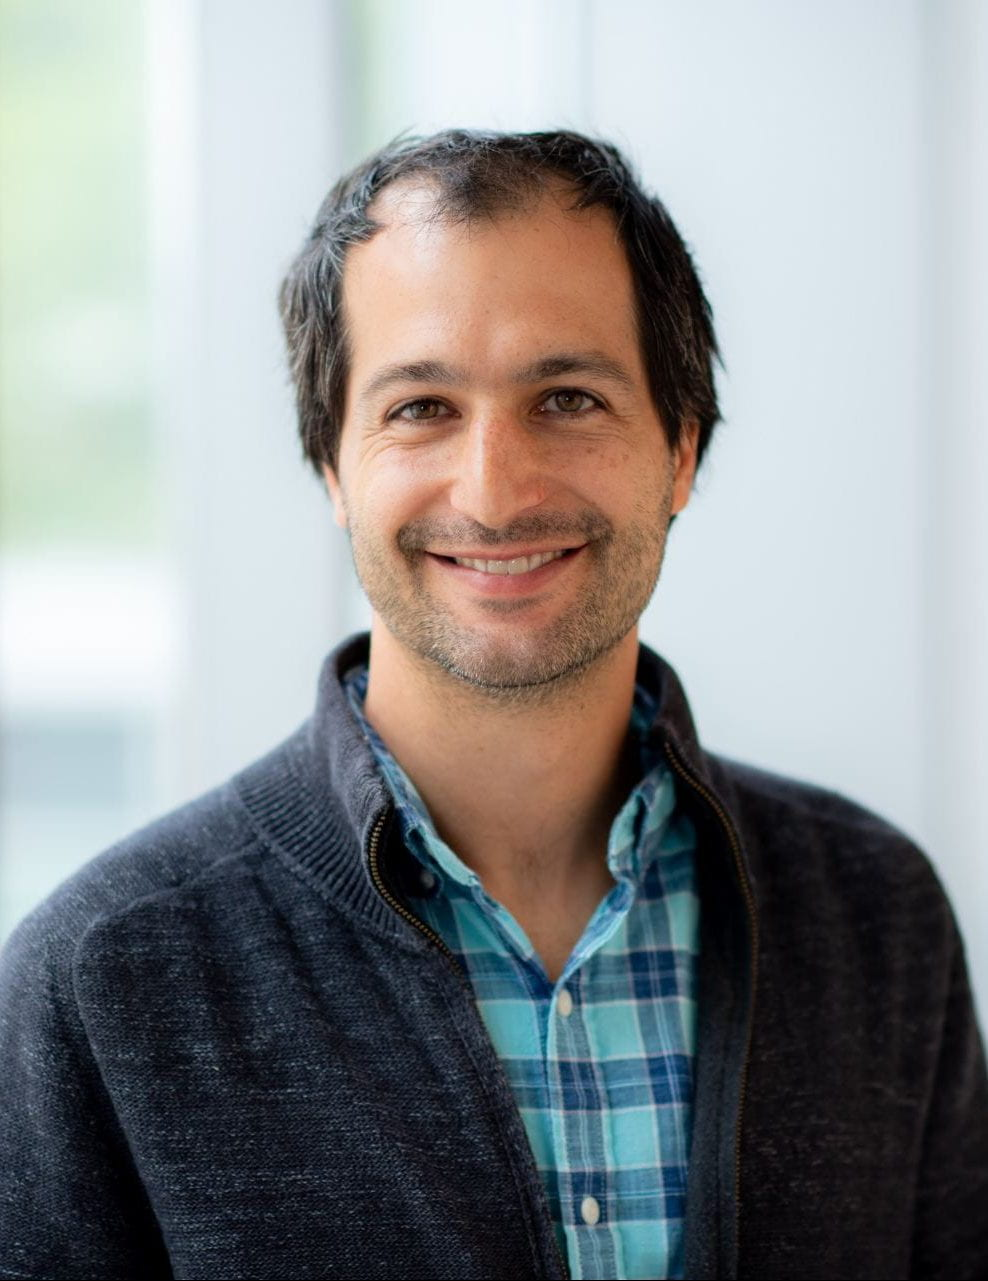
\includegraphics[height=2em]{img/matt-nassar.jpg}\\
\scriptsize
Matt Nassar
\end{minipage}
\begin{minipage}[t]{3em}
\center
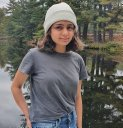
\includegraphics[height=2em]{img/niloufar-razmi.jpeg}\\
\scriptsize
Niloufar Razmi
\end{minipage}
\end{textblock}
\end{column}
\end{columns}
\end{frame}

\begin{frame}[label={sec:orgbf21ab9}]{Summary}
\end{frame}
\section*{Acknowledgments}
\label{sec:orga817e12}
{%
\setbeamertemplate{background canvas}{\includegraphics[height=\paperheight]{img/grand-canyon.JPG}}
\begin{frame}[fragile,t, plain]{Acknowledgments}
    \vspace{1em}
    \begin{columns}[T]
        \begin{column}{0.5\textwidth}
            \begin{itemize}
                \small
                \item Fleischmann lab~:
                \begin{itemize}
                    \tiny
                    \item Alexander Fleischmann
                    \item Keeley Baker
                    \item Olivia Mckissick
                    \item Tuan Pham
                    \item Simon Daste
                    \item Max Seppo
                    %\item \colorbox{white}{\transparent{0.2}Sara Zeppilli}}
                    \item Sara Zeppilli
                    \item Nell Klimpert
                    \item Erin Meyers
                    \item Eseosa Uwaifo
                    \item Camille Donoho
                    \item Timothy Pyon
                \end{itemize}
            \end{itemize}
        \end{column}

        \begin{column}{0.5\textwidth}
            \begin{itemize}
                \small
                \item Collaborations~:
                \begin{itemize}
                    \tiny
                    \item Jason Ritt (Carney Institute, Brown University)
                    \item Matt Nassar (Brown University)
                    \item Niloufar Razmi (Brown University)
                \end{itemize}
            \end{itemize}
        \end{column}
    \end{columns}
\end{frame}
}
\end{document}
